\subsubsection{Hidden Markov Model}
While Markov Models are very descriptive models of an environment often times when analyzing sound data we do not have the information to paint the full picture. Meaning we don't have the full sequence of states but we do have measurements from those states. Specifically, our states would be the specific sound that was made by an animal. We can call this a syllable (many bird songs consist of syllables). Sadly, we do not know these syllables we only know the acoustic signals that they produce. These signals would be the evidence or observation in our current definition of the HMM. Using the sound waves we translated via Fourier transform we can eventually get to the actual syllables made by the animal. 
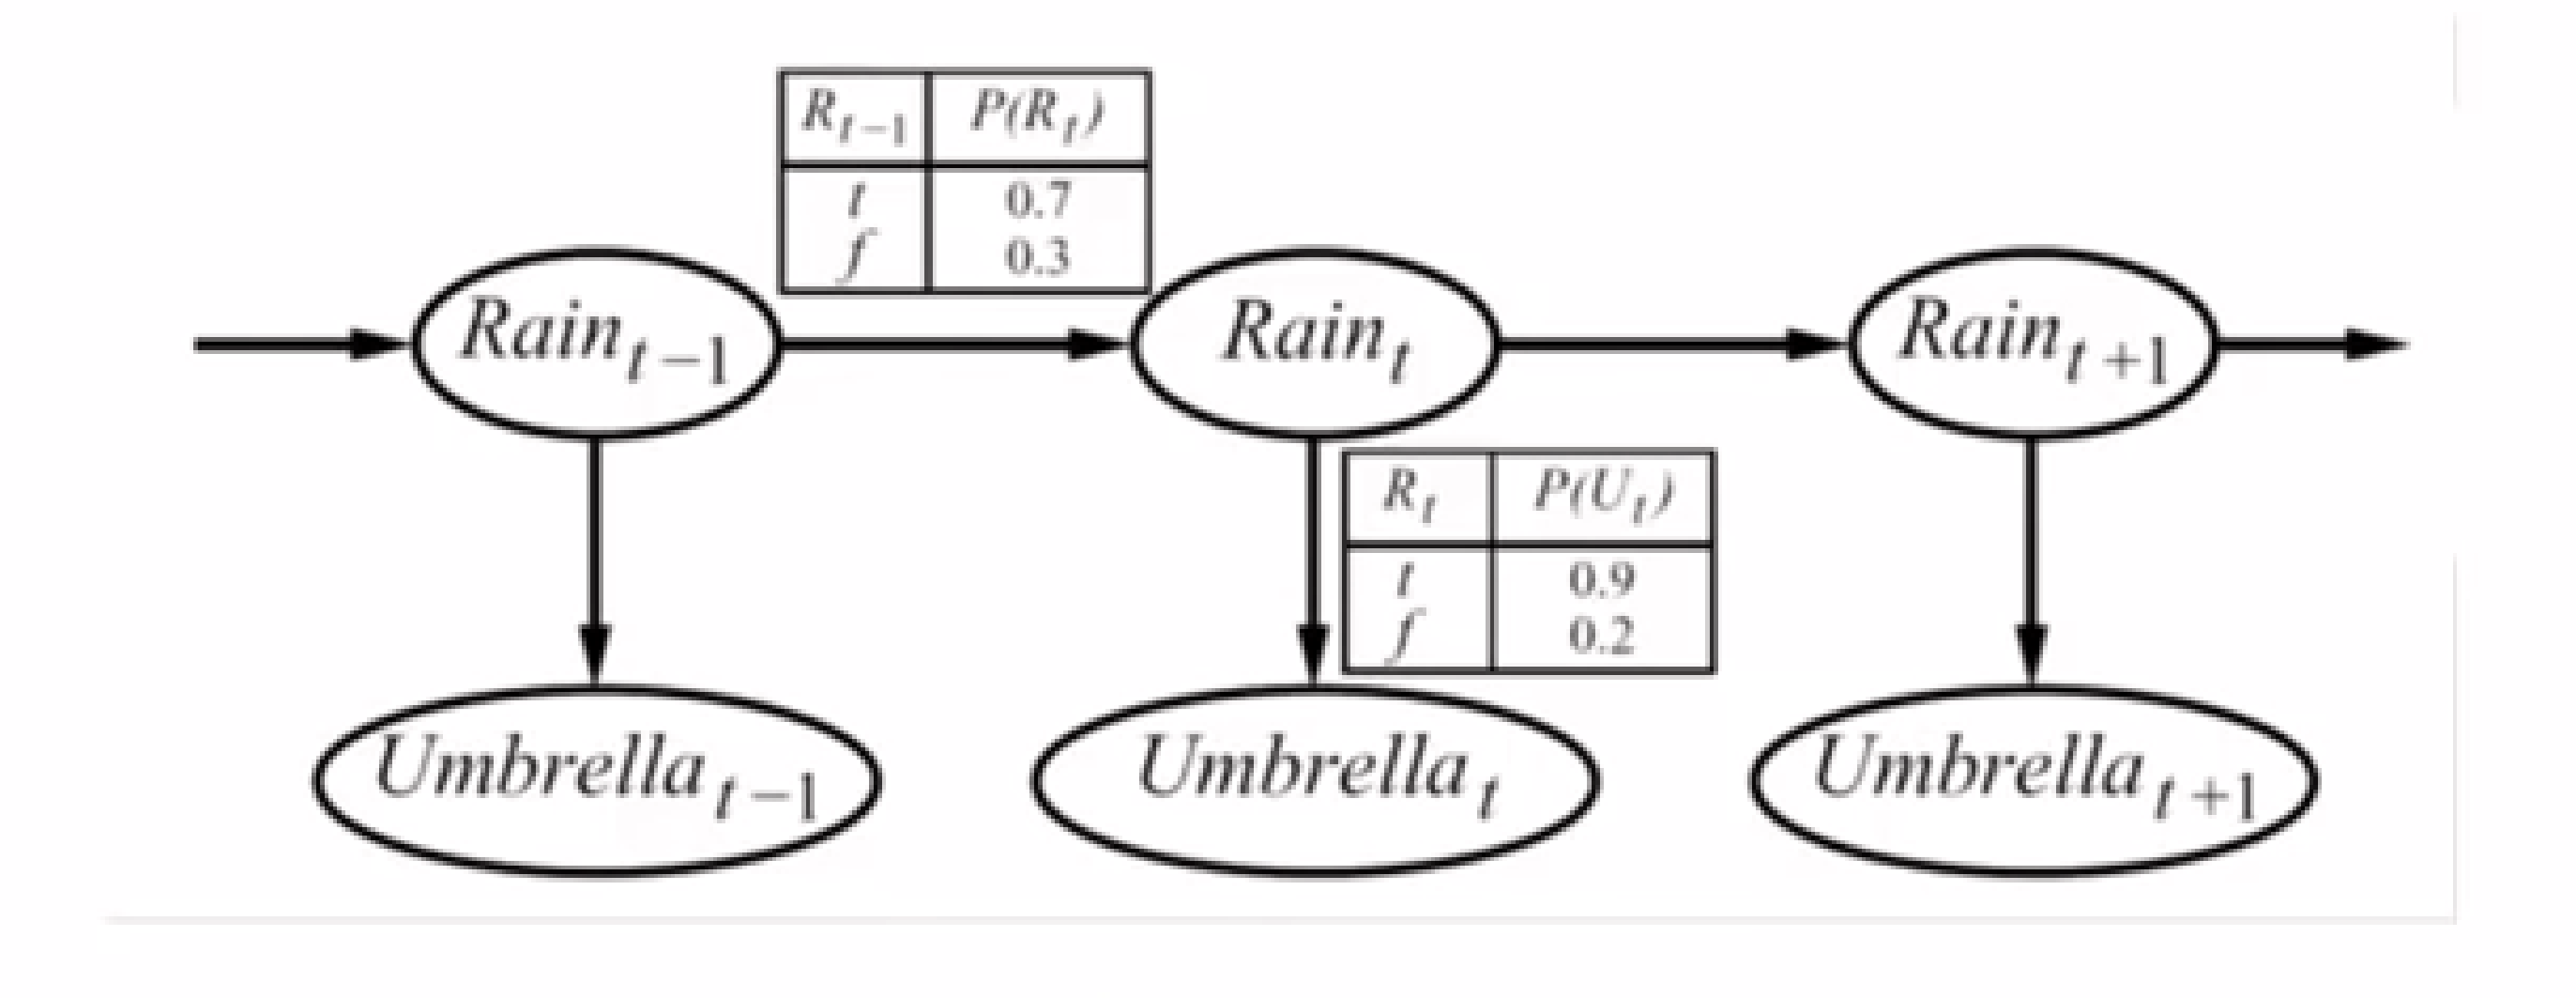
\includegraphics[width=\textwidth]{HMM}
When we talk about HMM we will talk about the belief the current system is in. This is in reference to running an inference of the state based on what kind on evidence we have received. An example would be figuring there is a \%60 chance that with the current configuration of sound waves that syllable A is the sound made by the bird. This belief is obtained by filtering the current state with previous evidence. This method can be described by the following:
\vspace{10px}
\begin{center}
	$B_{t}(X)=P_{t}(X_{t}|e_{1},...,e_{t})$ where e is the evidence and X is the current state.
\end{center}
\vspace{10px}
We then update the belief via the following function:
\vspace{10px}
\begin{center}
	$B'(X_{t+1})=P(X_{t+1}|e_{1},...,e_{t})=$$$\sum_{X_{t}}P(X_{t+1}|X_{t})P(X_{t}|e_{1},...,e_{t})$$
\end{center}
\vspace{10px}
Once we have an observation of the new evidence we include that into the model with the following function:
\vspace{10px}
\begin{center}
	$B'(X_{t+1})=P(X_{t+1}|e_{1},...,e_{t})=$$$\sum_{X_{t}}P(X_{t+1}|X_{t})P(X_{t}|e_{1},...,e_{t})$$
\end{center}
\vspace{10px}
We must then re-weight the likelihood of the current belief based on the probability of that belief state with the current evidence, using:
\vspace{10px}
\begin{center}
	$B'(X_{t+1})P(e_{t+1}|X_{t+1})$
\end{center}
\vspace{10px}
The following image shows how HMM's update their belief based of off time updates and then evidence updates.
\begin{center}
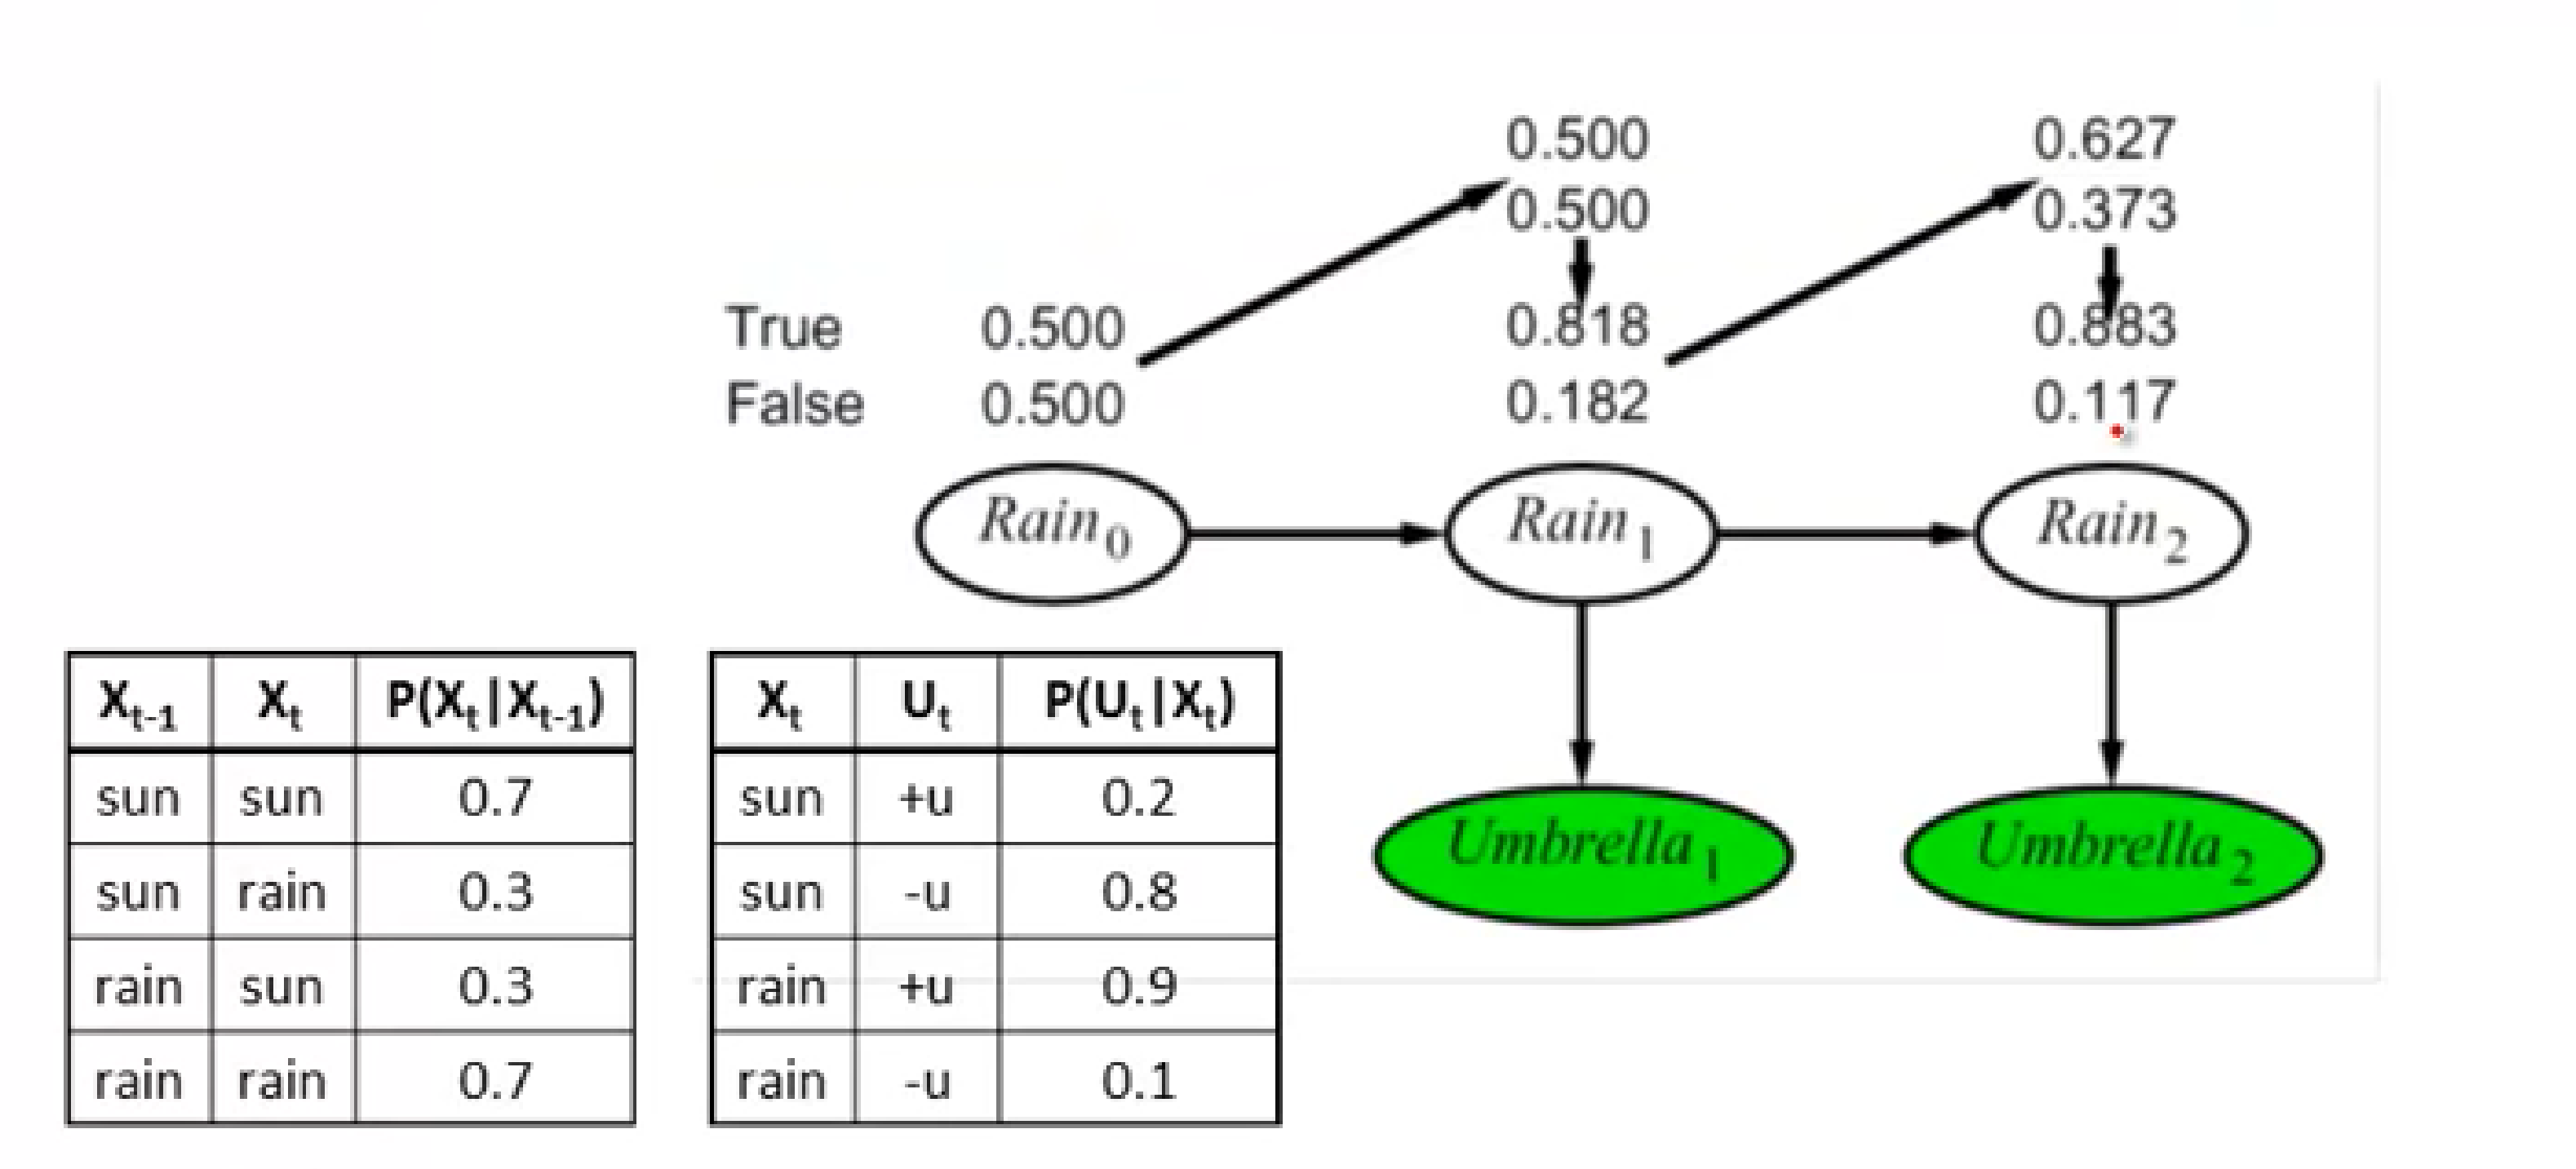
\includegraphics[width=\textwidth]{HMMupdate}
\end{center}
